\documentclass{article}

\usepackage[utf8]{inputenc}
\usepackage[french]{babel}

\usepackage{lmodern}
\usepackage{listings}
\usepackage{graphicx}
\usepackage{hyperref}
\usepackage{graphicx}
\usepackage{natbib}
\usepackage{tcolorbox}
\usepackage{xcolor}
\usepackage{array}
\usepackage{pifont}
\usepackage[a4paper, margin=1.5cm]{geometry}  
\usepackage{longtable}
\usepackage{float}
\usepackage{placeins}

\graphicspath{ {./res/} }
\author{
    Valentin Jonquière,
    Mathilde Chollon
}

\title{Rapport Architecture Logicielle}

\begin{document}

\maketitle

\pagebreak

\tableofcontents

\pagebreak

\section{Présentation du projet}

Ce rapport présente le projet du cours d'Architecture Logicielle de M1 Informatique à l'Université de Bordeaux.
Nous devions créer un logiciel de dessin vectoriel, où l'on peut manipuler différentes formes afin de créer des figures dans l'éditeur.
Le but de ce cours étant l'application de Design Patterns afin d'avoir une architecture propre, extensible et facilement maintenable, 
nous allons expliquer en section \ref{sec2} les patterns utilisés et leurs avantages pour notre implémentation.

Pour l'interface graphique, seulement quelques fonctions de \textit{Java AWT} étaient autorisées, comme les fonctions de dessin de rectangle, d'ovale ou de polygone, mais les types de formes devaient
être les nôtres.
Le logiciel présente plusieurs fonctionnalités clé qui sont les suivantes :
\begin{itemize}
    \item Sélection d'un objet depuis la toolbar et ajout au canevas via un glisser-déposer.
    \item Création/ suppression de groupes d'objets.
    \item Modification de la taille, position, couleur,... des objets.
    \item Ajout des formes crées à la toolbar via glisser-déposer.
    \item Annuler/ refaire une action.
    \item Sauvegarde/chargement d'un fichier contenant canevas et toolbar.
    \item Sauvegarde de la toolbar en quittant le logiciel, recharge au de celle ci au lancement.
\end{itemize}

\begin{figure}[h]
    \centering
    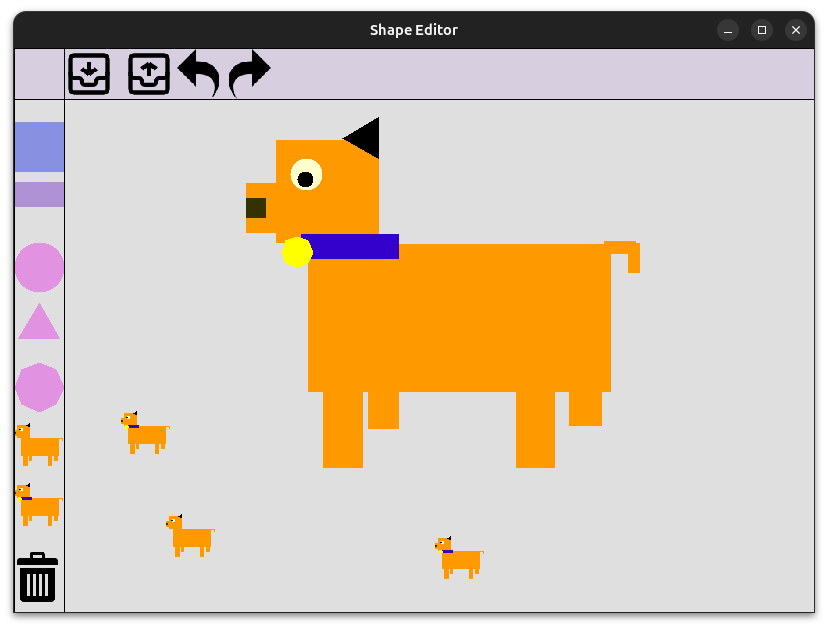
\includegraphics[width=0.8\textwidth,keepaspectratio]{dog.png}
    \caption{Exemple de dessin avec notre logiciel}
    \label{Clebs}
\end{figure}
\FloatBarrier
Sur la Figure \ref{Clebs}, on a un aperçu des différentes fonctionnalités du logiciel.
 Le chien a été créé à partir des formes basiques telles que le cercle, rectangle et polygone régulier.
 Grâce aux différentes possibilités d'édition de formes, nous avons pu changer la couleur, la forme ainsi que la tailles des formes pour créer le dessin voulu.
 On peut également voir que la forme a été ajoutée à la toolbar, et qu'il est possible de rajouter les formes de celles-ci au canevas.
 
\section{Design patterns utilisés} \label{sec2}

\subsection{Prototype}
Le pattern prototype a été utilisé dans les différentes formes en ajoutant une méthode \textit{clone()}. Cette méthode permet de faire une deep copy de l'objet,
 nous laissant modifier les champs du clone sans affecter ceux de la forme de base.
 L'interface Shape implémente \textit{Cloneable}, ce qui nous permet de créer ces clones.
 Toutes les implémentations concrètes de Shape implémentent clone() (tout sauf \textit{Polygon} et \textit{Ellipsoid}).
 Cela est particulièrement utile pour le drag-and-drop de la toolbar vers le canevas et inversement.

\subsection{Builder}
Nous avons choisi d'utiliser le pattern Builder afin de créer des fichiers de sauvegarde de l'état du logiciel. Cela nous permet de créer différentes implémentations
afin de sérialiser différents types de documents. Dans la Figure \ref{Builder}, nous pouvons voir que le \textit{FileBuilder} est l'interface contenant les différentes étapes de création
du fichier de sauvegarde. La classe \textit{XmlBuilder} correspond quant à elle au ``Concrete Builder'' du pattern, c'est-à-dire l'implémentation spécifique
de l'interface. Nous avons donc implémenté un builder de fichiers XML. Grâce à l'interface \textit{FileBuilder}, l'ajout de nouveaux builders concrets est facilitée.
Par exemple, il est possible de rajouter des savers au format txt ou JSON en implémentant l'interface \textit{FileBuilder}.
Ce qui va permettre la prise en charge différents formats de fichiers est le fait que la méthode \textit{getResult()} est présente uniquement dans les classes concrètes, ce qui ne va pas nous
limiter quant au format de retour des builders. Nous avons donc basé la structure de l'application sur le pattern Composite puisque notre modèle repose sur un Group nommé \textit{components}
comportant lui-même des groupes pour représenter la toolbar, le menu ou encore le canvas.

\begin{figure}[h]
    \centering
    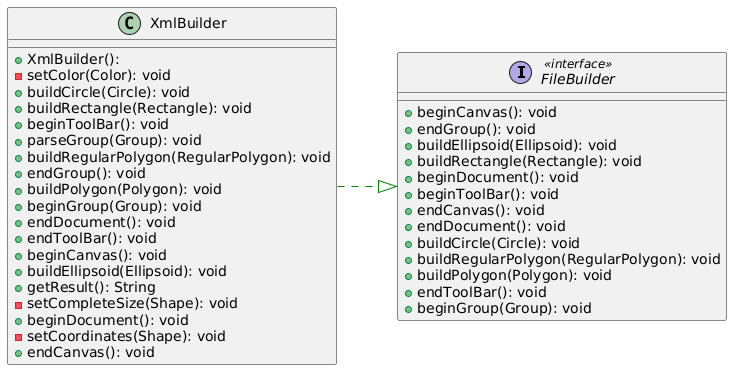
\includegraphics[width=\textwidth,height=5.0cm,keepaspectratio]{builder.png}
    \caption{Diagramme UML du Builder}
    \label{Builder}
\end{figure}
\FloatBarrier

Afin de rester cohérents lors du chargement de fichiers de sauvegarde, nous avons utilisé le même principe pour le Loader,
qui possède une interface \textit{FileLoader} ainsi qu'une implémentation concrète \textit{XmlLoader}.

\subsection{Composite}

Le pattern \textit{Composite} a été utilisé afin de simplifier la création de groupes de formes ainsi que de groupes de groupes de formes.
Les groupes devant posséder les mêmes traitements que les formes simples (resize, move, \ldots), la classe groupe implémentant également l'interface \textit{Shape}. Nous pouvons donc 
traiter de la même manière les groupes de formes et les formes individuelles telles que les polygones réguliers ou les cercles.  On utilise ici une liste couplée à un set de forme pour stocker
les formes contenues dans un groupe afin de pouvoir itérer facilement sur les éléments mais également garantir qu'une forme n'apparait qu'une fois dans un groupe grâce aux propriétés du set.
Nous possédons également un groupe particulier, la Toolbar. Elle possède les mêmes propriétés qu'un groupe, mais possède une fonction différente pour ajouter un nouvel élément. L'ajout est différencié
car il est nécessaire de pouvoir réorganiser l'agencement de la toolbar si une forme est supprimée par exemple (ne pas laisser un emplacement vide). Ce pattern est central à l'architecture de notre logiciel.
En effet, on peut considérer toute la fenêtre comme un ensemble de groupe. Dans le model, on retrouve le groupe \textit{components} représentant la racine. On peut ensuite ajouter les groupes toolbar, menu et
canvas représentant tous les trois des zones différentes de l'application avec des actions différentes (mouvement des formes sur le canvas, clique sur les boutons du menu, \ldots) pour définir l'aspect global de l'application. 
\begin{figure}[h]
    \centering
    \includegraphics[width=\textwidth,height=15.0cm,keepaspectratio]{Composite.png}
    \caption{Diagramme UML du Composite}
    \label{Composite}
\end{figure}
\FloatBarrier

\subsection{Singleton}

Le pattern \textit{Singleton} a été utilisé dans deux de nos classes. Premièrement, il a été utilisé dans la classe \textit{Model}, 
afin de garantir une instance unique, avec un point d'accès global au sein de l'application.
Cela nous permet par exemple de récupérer les formes présentes dans le canevas ou la toolbar, n'importe où dans l'application. Avec cette implémentation,
on peut utiliser une architecture MVC modifiée, où la Vue peut accéder au contenu du Modèle sans passer par le Contrôleur, ce qui évite l'envoi
de nombreuses commandes.
Le pattern a également été utilisé dans le \textit{BagOfCommands}. Celui ci remplace le Controller classique et permet d'exécuter des commandes (voir \ref{BoC}).

\begin{figure}[h]
    \centering
    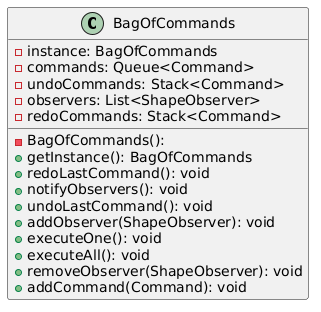
\includegraphics[width=\textwidth,height=5.0cm,keepaspectratio]{singleton.png}
    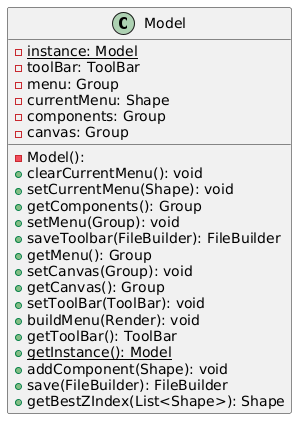
\includegraphics[width=\textwidth,height=5.0cm,keepaspectratio]{singleton2.png}
    \caption{Diagramme UML des deux Singleton}
    \label{Singleton}
\end{figure}
\FloatBarrier

Dans la Figure \ref{Singleton}, on peut voir que les deux classes possèdent un field privé \textit{instance}, du type de leur classe.
Leur constructeur est également privé. Ils possèdent tous deux la méthode publique et statique \textit{getInstance()} qui permet
d'accéder à l'instance unique de l'objet n'importe où dans le programme.

\subsection{Visitor}

\begin{figure}[h]
    \centering
    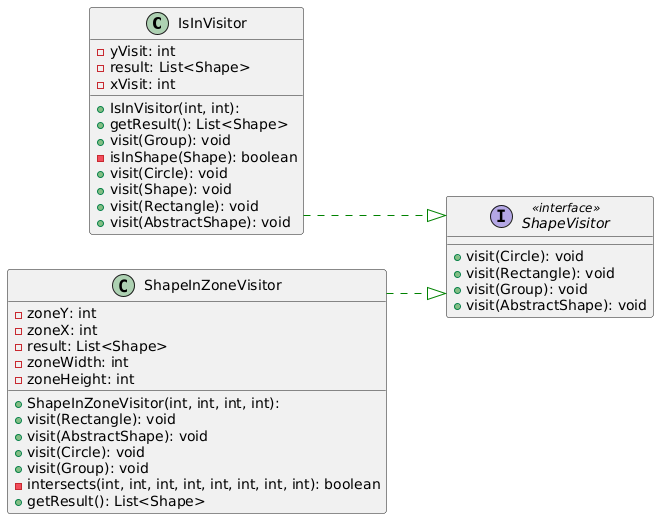
\includegraphics[width=\textwidth,height=10.0cm,keepaspectratio]{visitor.png}
    \caption{Diagramme UML du Visitor}
    \label{Visitor}
\end{figure}
\FloatBarrier
\subsection{Method factory}
Le pattern \textit{Method Factory} a été choisi afin de déléguer à d'autres classes la responsabilité de créer des éditeurs de formes
spécifiques à la forme créée. En effet, nous avions besoin de pouvoir instancier un éditeur différent pour chaque type de forme car elles
ne possèdent pas les mêmes traitements. Par exemple, il est possible de changer la couleur d'un cercle, d'un rectangle et d'un polygone régulier, mais pas celle d'un groupe.
Ici, le choix de l'éditeur à instancier est confié à la commande \textit{EditShapeCommand} car elle a accès à la forme à éditer. Les formes pouvant toutes
être re-dimensionnées, nous avons ajouté un \textit{AbstractEditor} afin de factoriser le code de cette opération et ainsi éviter la duplication de code.
De plus, les traitements pouvant être rangés par catégories (changement de couleurs, rotation, changement du nombre de coté), nous avons rassemblé les traitements
dans différentes classes capables de créer le menu d'édition pour son type d'opération dans le but d'éviter encore une fois la duplication de code.
\begin{figure}[h]
    \centering
    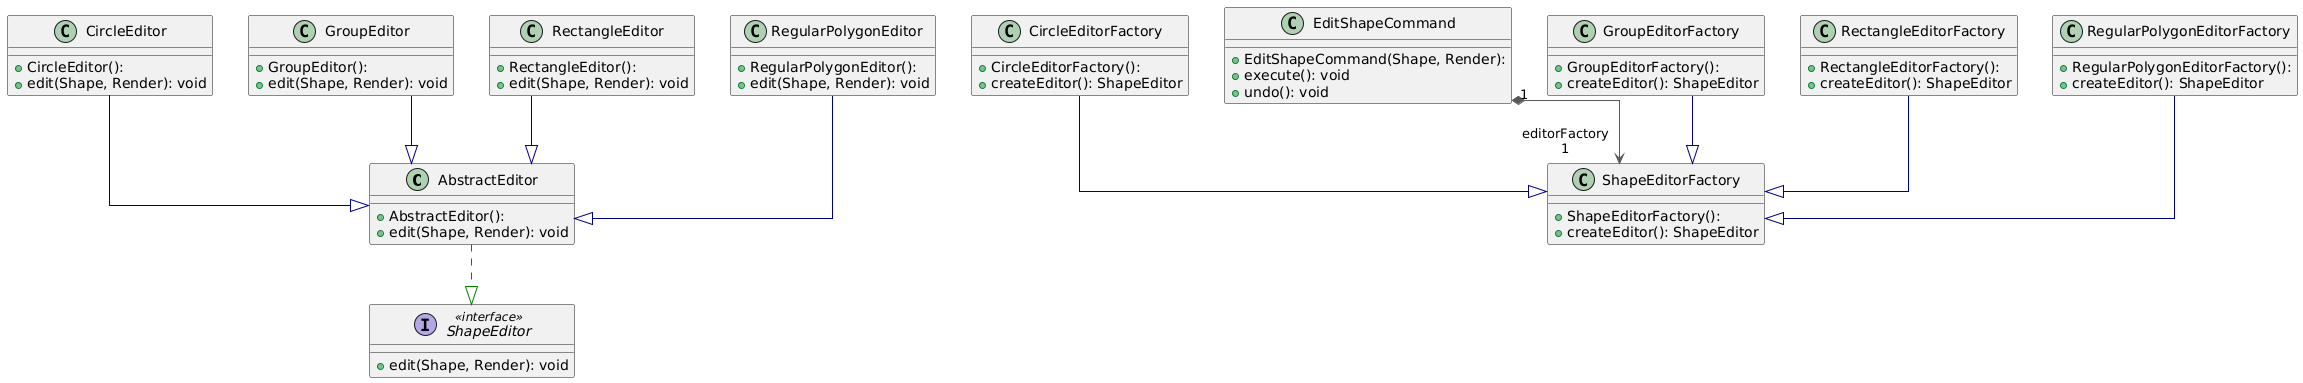
\includegraphics[width=\textwidth,height=10.0cm,keepaspectratio]{methodFactory.png}
    \caption{Diagramme UML de la Method Factory}
    \label{MethodFactory}
\end{figure}
\FloatBarrier
\subsection{Bridge}

Le pattern \textit{Bridge} a été choisi dans notre projet afin d'avoir la possibilité de changer de technologie dans notre vue
 sans modifier la logique de celle-ci. L'abstraction de la vue et son implémentation sont indépendantes.

Nous avons utilisé \textit{Java Awt} ici, mais il serait tout à fait possible d'utiliser \textit{JavaFX} ou d'autres frameworks graphiques
avec un minimum de modifications.

\begin{figure}[h]
    \centering
    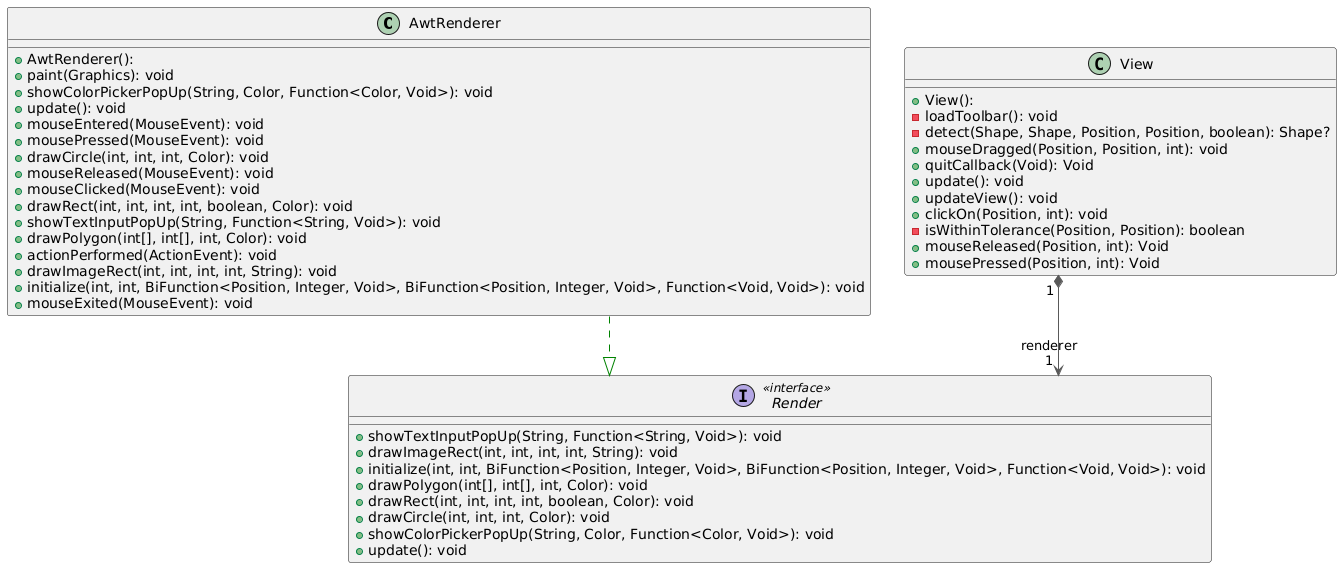
\includegraphics[width=\textwidth,height=10.0cm,keepaspectratio]{bridge.png}
    \caption{Diagramme UML du Bridge}
    \label{Bridge}
\end{figure}
\FloatBarrier

Sur la figure \ref{Bridge}, nous pouvons observer l'implémentation du Bridge via l'interface \textit{Render}.
La vue va communiquer avec celle-ci, ce qui abstrait l'utilisation d'une technologie particulière.
La classe \textit{AwtRenderer} est une implémentation concrète de l'interface \textit{Render}. 
Tout le code spécifique à JavaAWT se situe dans cette classe, ce qui ne soumet pas l'application à
l'utilisation de cette technologie de rendu graphique.
La classe \textit{View} est quant à elle l'abstraction du pattern, elle utilise un objet de type \textit{Render} sans se soucier de son implémentation concrète.

Ce choix d'architecture nous permet d'implémenter indépendamment la vue du render, ce qui nous permettrait de rajouter d'autres
implémentations concrètes de ce dernier sans affecter la vue.
On découple totalement l'abstraction de l'implémentation.
\FloatBarrier
\subsection{Observer}
\begin{figure}[h]
    \centering
    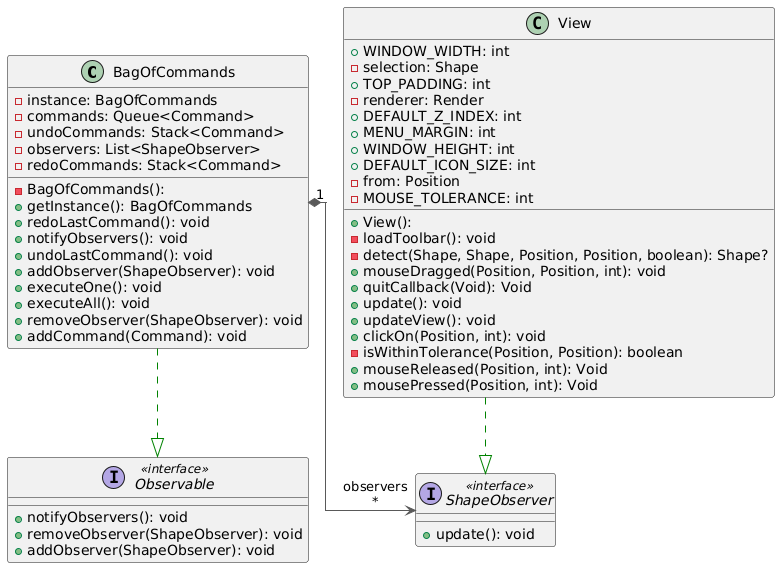
\includegraphics[width=\textwidth,height=10.0cm,keepaspectratio]{observer.png}
    \caption{Diagramme UML de l'Observer}
    \label{Observer}
\end{figure}
\FloatBarrier

\subsection{Memento}
\begin{figure}[h]
    \centering
    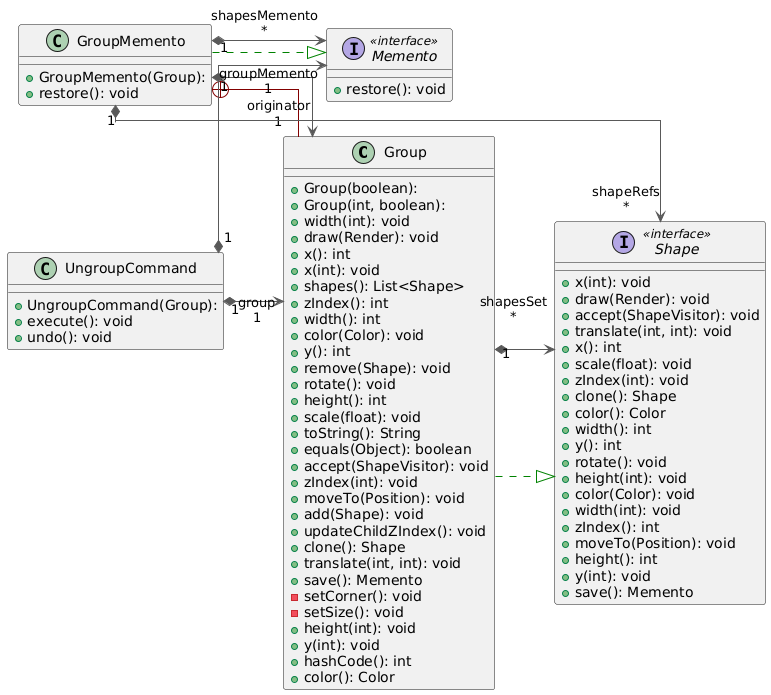
\includegraphics[width=\textwidth,height=10.0cm,keepaspectratio]{memento.png}
    \caption{Diagramme UML du Memento pour un groupe}
    \label{MementoGroupe}
\end{figure}
\FloatBarrier

\begin{figure}[h]
    \centering
    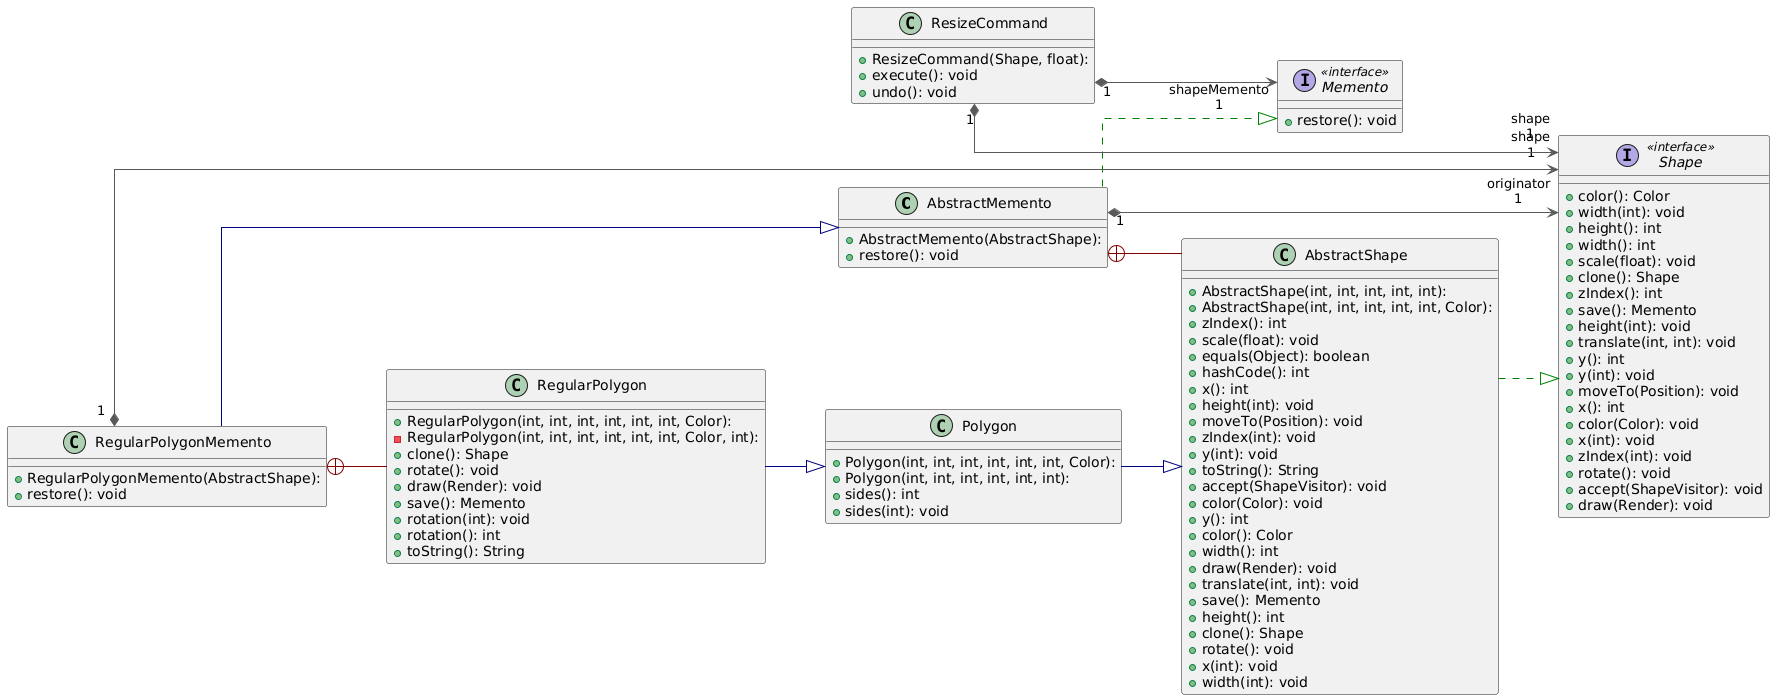
\includegraphics[width=\textwidth,height=10.0cm,keepaspectratio]{memento2.png}
    \caption{Diagramme UML du Memento pour une forme simple}
    \label{MementoShape}
\end{figure}
\FloatBarrier

\subsection{Command + Bag Of Command} \label{BoC}

\begin{figure}[h]
    \centering
    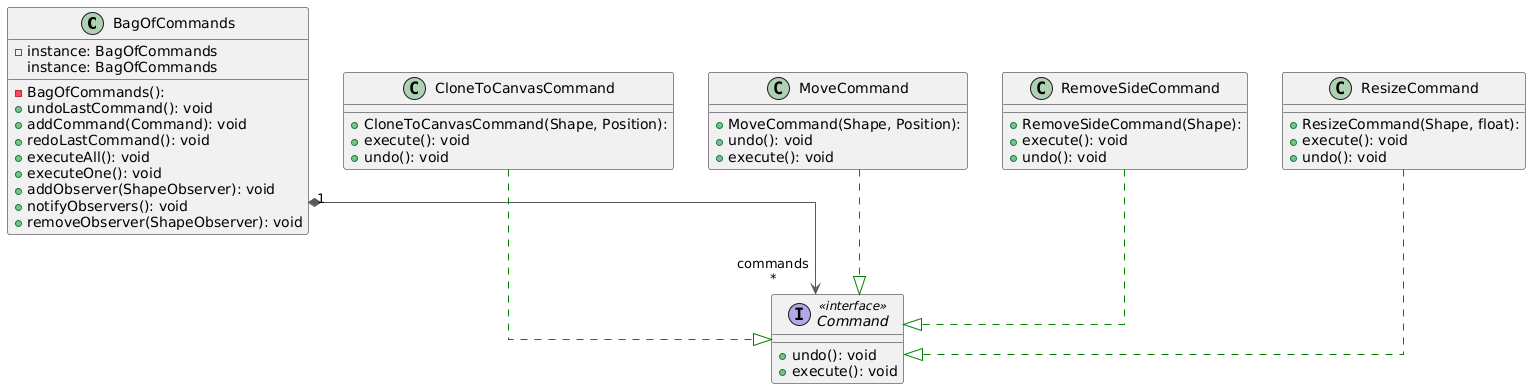
\includegraphics[width=\textwidth,height=10.0cm,keepaspectratio]{command.png}
    \caption{Diagramme UML des Commandes}
    \label{Command}
\end{figure}
\FloatBarrier

\end{document}